\documentclass[10pt]{article}

% amsmath package, useful for mathematical formulas
\usepackage{amsmath}
% amssymb package, useful for mathematical symbols
\usepackage{amssymb}

% graphicx package, useful for including eps and pdf graphics
% include graphics with the command \includegraphics
\usepackage{graphicx}

% cite package, to clean up citations in the main text. Do not remove.
\usepackage{cite}

\usepackage{color} 

% Use doublespacing - comment out for single spacing
\usepackage{setspace} 
\doublespacing

% Text layout
\topmargin 0.0cm
\oddsidemargin 0.5cm
\evensidemargin 0.5cm
\textwidth 16cm 
\textheight 21cm

% Bold the 'Figure #' in the caption and separate it with a period
% Captions will be left justified
\usepackage[labelfont=bf,labelsep=period,justification=raggedright]{caption}

% Use the PLoS provided bibtex style
\bibliographystyle{plos2009}

% Remove brackets from numbering in List of References
\makeatletter
\renewcommand{\@biblabel}[1]{\quad#1.}
\makeatother


% Leave date blank
\date{}

\pagestyle{myheadings}
%% ** EDIT HERE **

\usepackage{multirow}

%% ** EDIT HERE **
%% PLEASE INCLUDE ALL MACROS BELOW

% figure files reside in the figures/ directory
\graphicspath{
{figures/}
}

%% END MACROS SECTION

\begin{document}

% Title must be 150 characters or less
\begin{flushleft}
{\Large
\textbf{Spatially explicit model of the lymphocyte diaspora in influenza-infected lung quantifies constraints of chemokine directed migration (SUPPLEMENT)}
}
% Insert Author names, affiliations and corresponding author email.
\\
Drew Levin$^{1,\ast}$, 
Stephanie Forrest$^{1}$, 
Soumya Banerjee$^{1}$
Candice Clay$^{2}$, 
Melanie Moses$^{1}$, 
Frederick Koster$^{2}$, 
\\
\bf{1} Department of Computer Science, University of New Mexico, Albuquerque, NM, USA
\\
\bf{2} Lovelace Respiratory Research Institute, Albuquerque, NM, USA
\\
$\ast$ E-mail: Corresponding drew@cs.unm.edu
\end{flushleft}


% You may title this section "Methods" or "Models". 
% "Models" is not a valid title for PLoS ONE authors. However, PLoS ONE
% authors may use "Analysis" 
\section*{Models}


\subsection*{Ordinary Differential Equation Models}

To find a value for $\sigma$ we use a differential equation model from \cite{Miao20101}:

\begin{equation*}
\begin{aligned}
\frac{dN_{c}}{dt} &= \sigma - \frac{r'^{2} \cdot N_{c}}{R^{2} \cdot t_{rc}}    & \pi r'^{2} &= a \sqrt{I} + b \\
\frac{dN'_{f}}{dt} &= \frac{(r'^{2} - r^{2}) \cdot N_{c}}{R^{2} \cdot t_{rc}} - \frac{v_{tcell}}{(r' - r) / 2} \hspace*{2cm}  & \pi r^{2} &= \pi r_{cell}^{2} \cdot I \\
\frac{dN_{f}}{dt} &= \frac{r^{2} \cdot N_{c}}{R^{2} \cdot t_{rc}} + \frac{v_{tcell}}{(r' - r) / 2} \\
\frac{dT}{dt} &= \rho T -\beta TV \\
\frac{dI}{dt} &= \beta TV - \delta I - k_{e} N_{f} I \\
\frac{dV}{dt} &= pI - \beta TV - \gamma (t) V \\
\gamma (t) &= \left\{ \begin{array}{rcl}
	1/\mbox{day} & \mbox{,}  & t < 5  \\
	3/\mbox{day} & \mbox{,} & t \geq 5  
	\end{array}\right. \\
\end{aligned}
\end{equation*}


where $N_{c}$ is the number of circulating activated antigen-specific T-cells, $N'_{f}$ is the number of circulating T-cells that have found and exit into a region of lung tissue expressing chemokines and $N_{f}$ is the number of circulating T-cells that have found an infected region. $T$ is the number of uninfected target cells, $I$ is the number of productively infected cells, and $V$ is the viral titer in serum. The infected region is assumed to be of radius $r$ and is within a region expressing chemokines of radius $r'$ ($r  < r'$). The lung is assumed to be a circular region with radius $R$. The area of the infected region is equal to the area of an infected cell (of radius $r_{cell}$) multiplied by the number of infected cells. The area of the region expressing chemokine was found to be related non-linearly to the number of infected cells ($\pi r'^{2} = a \sqrt{I} + b$) where $a$ and $b$ are constants that depend on the viral strain.

Circulating activated antigen-specific T-cells ($N_{c}$) are assumed to be released from lymph nodes at a constant rate $\sigma$. These circulating cells then transition into $N'_{f}$ and $N_{f}$ at rates proportional to the areas of the chemokine expressing and infected regions relative to the whole lung area. Circulating cells that are in the chemokine expressing region ($N'_{f}$) transition to the infected region after walking randomly for an average time proportional to the difference in the radii between the two regions ($r' - r$). Target cells ($T$) become infected by virus at rate $\beta TV$, where $\beta$ is the rate constant characterizing infection. Infected cells ($I$) die at rate $\delta$ in addition to being lysed by T-cells ($N_{f}$) at a rate $k_{e}$. Finally the viral titers ($V$) increase due to production of virus at rate $p$ by infected cells. Virus is also cleared due to uptake by infected cells (at a rate $- \beta TV$) and due to antibody (at a rate $\gamma (t)$ that changes after 5 days post infection). The initial viral titer and the initial number of target cells are denoted $V_{0}$ and $T_{0}$, respectively. The initial number of infected cells is assumed to be zero. This ode was fit to data taken from \cite{Miao2010} using Matlab's \texttt{nlinfit} function in order to obtain a value for $\sigma$.

% Results and Discussion can be combined.
\section*{Results}

\subsection*{Stochastic modeling effects}

Unlike ODE models, which are deterministic, stochastic models such as CyCells can produce different results on different runs (Figure~\ref{fig:variance}).  To test the strength of this effect, we ran each model fifty times using the default parameters given in Table~\ref{table:parameters}.  $R^2$ values were calculated for individual runs versus the average of all runs.  Pandemic H1N1 showed the least inter-run variance with an mean $R^2$ value of 0.9935 and standard deviation of 0.0029.  sH1N1 had a mean $R^2$ 0.9859 with a standard deviation of 0.0109.  aH5N1 had a mean $R^2$ of 0.9167 with a standard deviation of 0.0726.  

Each run took the calculated viral production and chemokine production rates for the three different strains of influenza as input and reported the total number of infected cells, including incubating, virus secreting and apoptotic, but not including dead cells.  Therefore the figures approximate plaque growth over time.

Overlaying multiple runs on a single plot reveals a slight growth rate transition 3 days p.i., which reflects the addition of IgM.  In addition, for each infection the number of infected cells declines quickly at day five due to the T-cell response. 

The three strains show different levels of virulence, consistent with the results found in \cite{Mitchell2011} (Fig.~\ref{fig:variance}).  The rapid growth of the pandemic H1N1 prevents the immune response from containing the infection.  Because pH1N1 is replicates at such a rapid rate, the window of opportunity for T-Cells to gain ground is too small.  aH5N1 is cleared completely, sH1N1 is contained but not fully cleared, and pH5N1 recovers and continues to expand.

\begin{figure}[ht!]
\begin{center}
 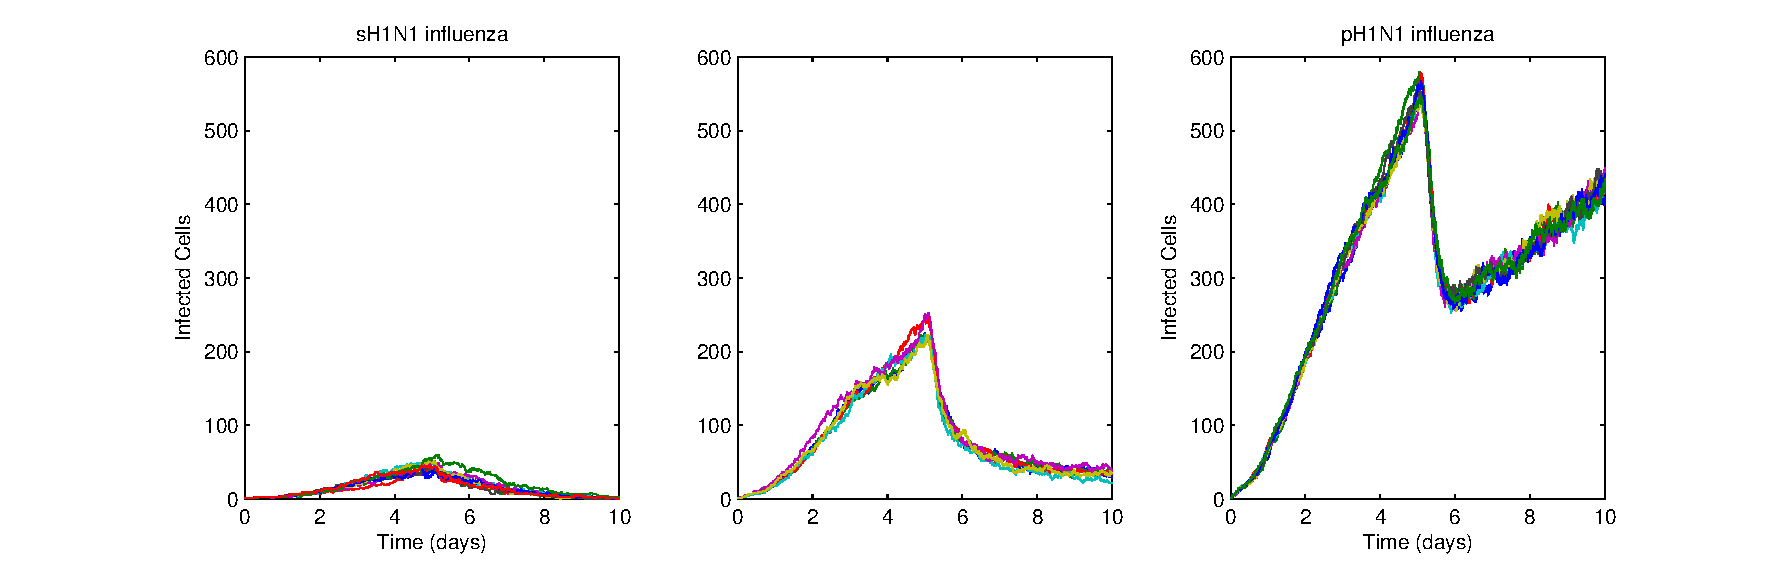
\includegraphics[width=\textwidth]{variance}
 \end{center}
\caption{Model results: Time series plots of fifty runs of aH5N1 (A), sH1N1 (B), and pH1N1 (C) infections (gray). IP-10 and RANTES were simulated in each run, except for aH5N1, which  produced only RANTES.  Each run was initialized identically for each strain save for the random seed.  The middle line shows the average while the outer lines show the 95\% confidence interval.} 
 \label{fig:variance}
\end{figure}


\subsection*{Chemokine combinations}

Because aH5N1 has been shown to suppress the production of interferon \cite{Mitchell2011}, we hypothesize that it renders IP-10 ineffectual.  We hypothesize that this leads to the elevated RANTES secretion rates measured in aH5N1 compared to the other two strains (Table~\ref{table:strains}).  Because of this behavior IP-10 was not included in the aH5N1 model runs.-
Four models runs were performed for each strain (two for aH5N1) to look at how the presence and/or lack of specific chemokines affect the simulated immune response (Fig.~\ref{fig:chemokine}).  The lack of both chemokines leads to runaway infections in all three strains.  The presence of only RANTES is enough to contain the aH5N1 infection, but is weaker than IP-10 in both H1N1 strains.  IP-10 alone proves to be as effective as the combination of IP-10 and RANTES, suggesting that RANTES does not play a significant role in infections that stimulate an IP-10 response.

\begin{figure}[ht!]
\begin{center}
	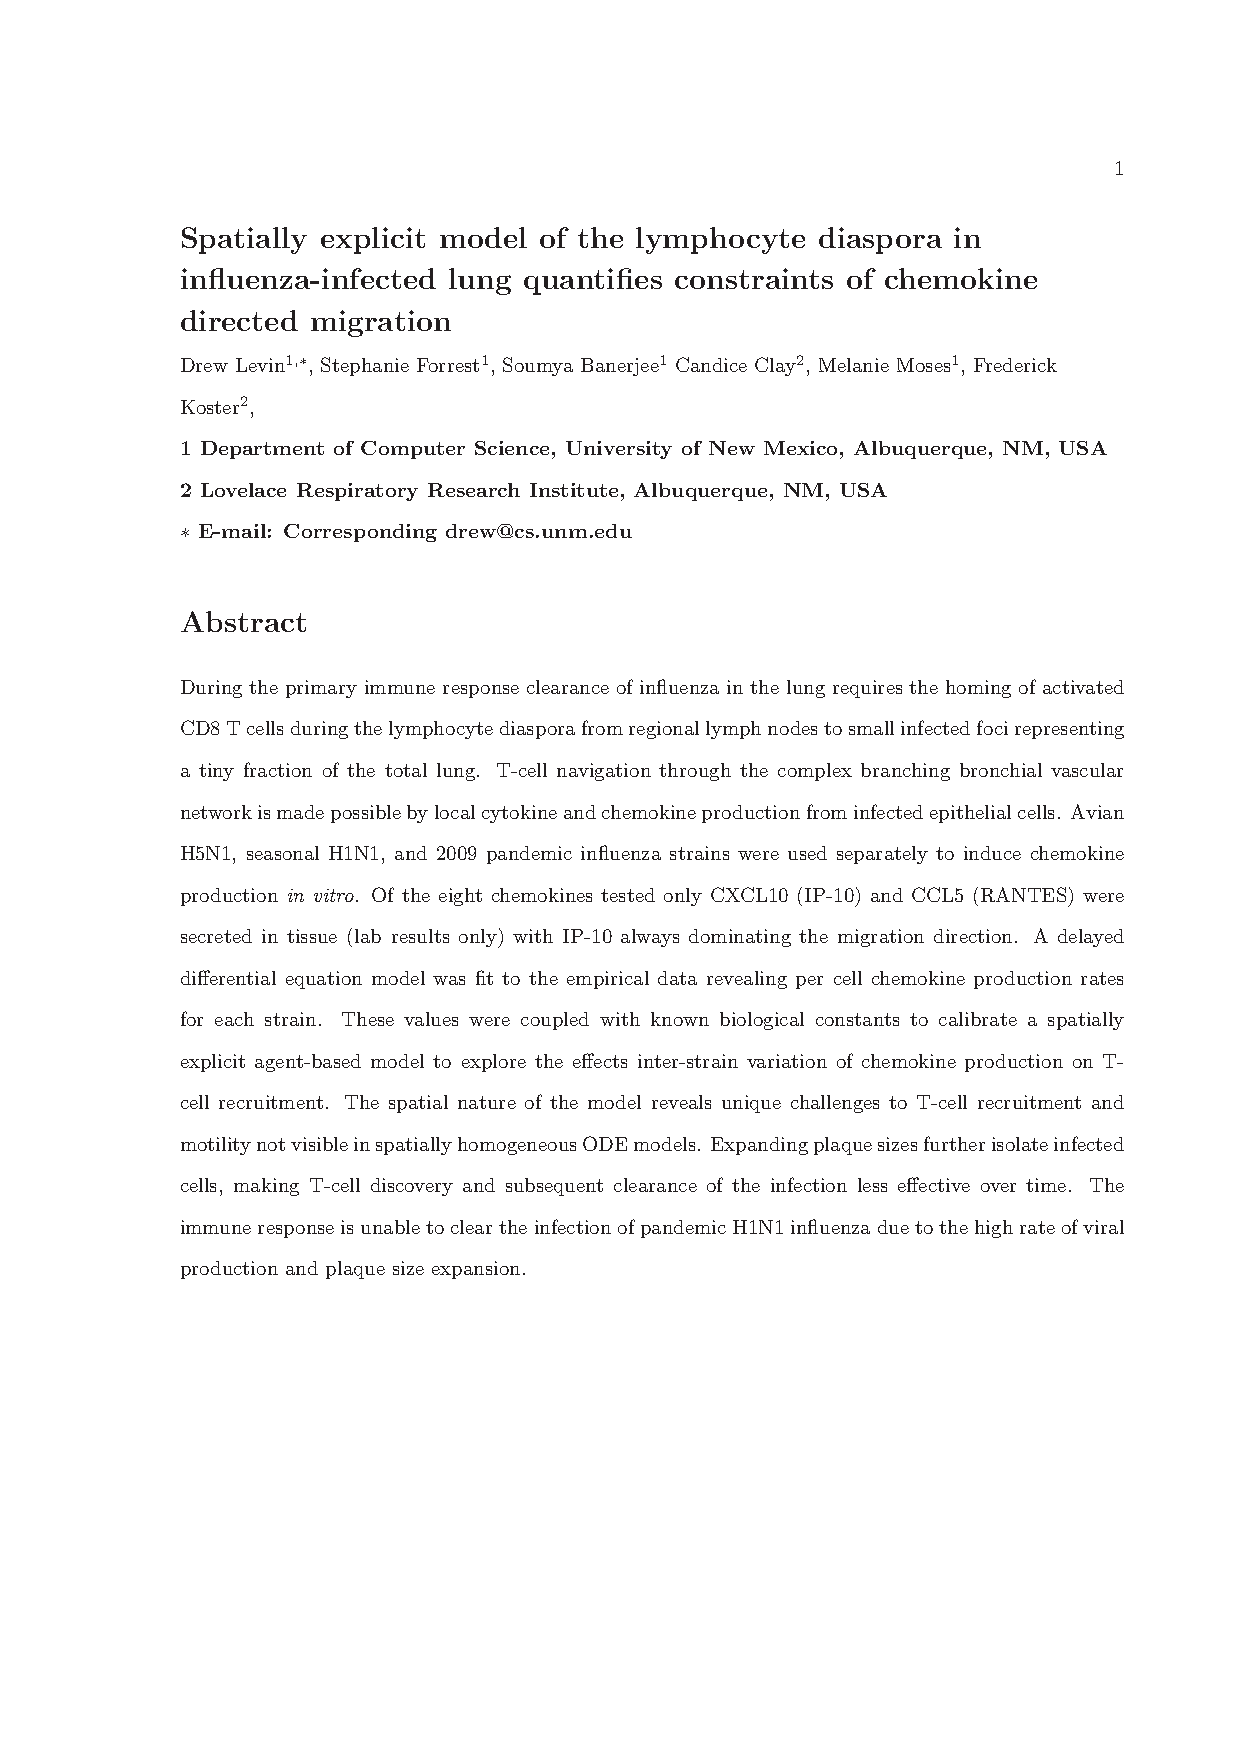
\includegraphics[width=\textwidth]{chemokine}
	\caption{Effects of different chemokine combinations.  A) aH5N1 does not stimulate an IP-10 response.  B-C) sH1N1 and pH1N1 show no significant difference between IP-10 alone versus IP-10 and RANTES combined.}
	\label{fig:chemokine}
\end{center}
\end{figure}



\section*{Miscellaneous Text}

\subsection*{General Immune Response Modeling}

The adaptive immune response to influenza in the mouse is a complex network of molecular and cellular elements, and incorporation of all of these into a comprehensive predictive model is not yet achieved.  Recent whole-animal models using a data-fitting approach and extensive databases have enhanced our global understanding of response metrics that are difficult or impossible to measure.  We have focused exclusively on the problem of the search of activated CTL for infected foci in the lung, and as in other models have made a number of assumptions.

The generally held view of the sequence of CD8+ T cell events during a primary immune response to influenza in the lung involves the following steps: dendritic cells bearing specific antigen migrate from the lung to the draining lymph node where naïve precursors are encountered and activated.  T cells proliferate in the lymph node and are released into the bloodstream, appearing simultaneous in the lung, spleen and other organs 4-5 days post-infection after to extravasation from the blood [Marshall 2001].   In the lung, extravasation from capillaries is signaled by inflammatory cytokine-mediated integrin-activation on endothelial cells.  Once in the tissue, T cells are guided up a chemokine gradient to the infected epithelial cell secreting the chemokine.  One of the model simplifications we utilized was the equating cytokine and chemokine signals.

A large fraction of the T cells entering lung tissue have come from the spleen where they proliferated under stimulation from antigen-loaded DC.  This has been demonstrated by the significant loss of T cells entering lung following splenectomy differential [Tripp 1997] and by math modeling results that make sense only if there is a significant proliferation of activated cells outside the lymph node prior to arrival in the lung [Wu 2011].  Our model did not include the proliferation in the temporary splenic reservoir as this uncertain degree of time delay in arrival between LN and lung would have complicated our ABM model.  Using numbers of cells egressing from LN likely underestimated the rate of CTL population entering the lung, but our derivations of parameters impacting the T cell search and subsequent function are probably not affected.

The fundamental mechanisms regulating the expansion of viral load and subsequent clearance of virus remain unclear, with current hypotheses focusing on antigen-driven, target cell susceptibility-driven, innate immune response-driven, antigen presentation limited, and adaptive immunity responses.  We used the data from strain-specific viral replication in vitro in human bronchial epithelial cells [Mitchell 2011] to structure the regulation of viral abundance and viral clearance as essentially a model of antigen-driven, innate immunity-driven regulation.  In a differential equation model, regulation of viral load was primarily driven by the availability of susceptible target cells [Baccam 2006].  The question of target-driven versus antigen-driven regulation was addressed in a separate modeling study of infected equine lungs [Saenz 2010], finding that regulation was primarily innate immunity-driven since no more than 27\% of bronchial epithelial cells were ever infected during the course of the lung infection.  In a comprehensive model of murine influenza rate-limiting antigen presentation was the primary influence on viral clearance [Lee 2009].  In a subsequent model based on a large murine database, CD8+ T cells were critical components of the adaptive response in limiting the number of infected cells, with neutralizing antibodies responsible for clearing free virus [Miao 2010].   Most modeling studies used a mouse-adapted virus to enable enumeration of epitope-specific T cells, making direct comparisons of replication efficiency with our human virus isolates more difficult.  The mechanism of regulation of animal viral load may be specific to viral replication efficiencies, strain-specific suppression of innate immunity, and the phase of the immune response.  We compared the three strains for their demands placed on the T cell search mechanism to find and kill infected cells. The multiplicity of potential regulation mechanisms does not invalidate our approach to the T cell search mechanisms. 

Our focus on the T cell search necessitated the simplification or removal of selected features of the mammalian immune response, in order to permit tractable simulations.  Antigen presentation and peripheral lymphoid tissue amplification of the T cell clonal response is represented solely by the constant rate of emigration of activated T cells from regional lymph nodes.  Virus-specific strain replication rates are represented as constant rates, and virus clearance is also constant.  The contribution of IgM antibody clearing free virus is represented at a constant rate, and the class switch to higher affinity antibody mediated by CD4+ T cells is not represented.  All of these rates may in fact be time-variable rates as indicated by superior data-fitting models [Wu 2011].  Immigration and contributions of virus-nonspecific immune cells such as macrophages are not represented in our model.  Finally, the proliferation of activated T cells in lung tissue is not represented, but is thought to be crucial in the control of lung infection [Miao 2010].  Since known critical components were omitted or simplified, our model was not designed to demonstrate clearance of virus from the lung.  Rather our goal was to examine the features of the response that permitted T cells to sense and contact infected target cells.


\subsection*{Chemokine Directed T-cell Search}

Hypercytokinemia is a characteristic of virulent influenza strains \cite{DeJong2006} but bloodstream levels of cytokines and chemokines may not reflect local concentrations and dynamics critical in guiding T cells to infected epithelial cells.  We elected to use our data on in vitro secretion of chemokines by human bronchial epithelial (NHBE) cells obtained from the same cultures of the three virus strains previously reported \cite{Mitchell2011}.  In this study the replication kinetics and productivity of the three virus strains were markedly different, but monolayer infection was initiated with a low MOI of 0.01 or 0.001, mimicking the initial infection naturally.  The levels of the chemokines CCL5 and CXCL10 in the basal media induced by the 3 strains were approximately equivalent at 24h post-infection.  When the productivity per cell was calculated, the avian H5N1 strain induced higher secretion of CCL5 (RANTES) than the seasonal or pandemic strains.  Greater CCL5 secretion by H5N1 strains has been noted in in vitro NHBE cultures when a relatively high MOI is used compared to seasonal strains \cite{Chan2005, Chan2010, Zeng2011} and pandemic strains \cite{Zeng2011}.  MOI and degree of differentiation of NHBE are critical determinants of cyto/chemokine secretion \cite{Chan2010}.  However, in spite of the attenuated type 1 interferon response induced by H5N1 strains \cite{Zeng2007}, the chemokine secretion is not attenuated.

Chemokines with a clear role directing T cell traffic include CXCL10 \cite{Dufour2002}, CCL5 \cite{Kawai1999} and CCL3 \cite{Kawai1999}.  The chemokine receptor CCR5, binding CCL5 and other chemokines, is crucial in the accelerated recruitment of CD8+ T cells to lung airways \cite{Kohlmeier2008}.  Other chemokines are likely to play a role in T cell traffic.  Although we did not detect significant levels of other chemokines in our cultures, the neutrophil- and T cell-attractant CXCL8/IL-8 is secreted into seasonal influenza-infected NHBE cultures \cite{Matsukura1996, Arndt2002}.  In the intact animal immigrant inflammatory cells particularly macrophages augment the multiple chemokine signals \cite{Julkunen2000}.  Finally, antigen-specific CD8+ T cell recognition of its target will induced lung injury mediated by TNFa and trigger addition alveolar epithelial cell chemokine secretion \cite{Zhao2000}.   Thus our model represents only a portion of the complete chemokine signal complex operating in the infected animal.

A key determinant in the efficiency of chemokine-directed T cell migration towards virus-secreting epithelial cells is the communication distance, defined by the threshold of sufficient chemokine signal to induce directed motion of the cell up the chemical gradient \cite{Thelen2008}.  The diameter of this cloud generated by a single cell is a function of production rate, decay rate, protein diffusion and the sensitivity threshold.  For the threshold of 100 pg/mL and maximal levels of concentration in tissue of 10,000 pg/mL, we calculated the effective communication distance as approximately 250 microns in our model.  This calculation matches the distance calculated for generic cytokines secreted by a suspended solitary cell \cite{Francis1997}.

NEW

In our model directed migration and viral infection control was not limited over a wide range of T cell sensitivity to the chemotactic signal.  The density of CCR5 receptors on the surface of CD8+ T cells was a determinant of the strength of chemotactic attraction for CCR5 ligands such as CCL5 in an in vitro assay [Desmetz 2006].   The density of CCR5 receptors on human CD8+ T cells vary over an order of magnitude, suggesting that sensitivity to the chemotactic signal could play a role in susceptibility to infection.  CCR5-knockout mice are susceptible to fatal Cryptococcal encephalitis/meningitis [Huffnagle 1999] and West Nile virus encephalitis [Glass 2005].  In the Cryptococcus-infected mice T cell recruitment to the brain, but not to the lung, was impaired.   In CCR5-KO mice influenza A virus pneumonia was more severe associated with decreased T cell recruitment to the lung, while in CCR2-KO mice decreased T cell recruitment was due to decreased macrophage influx into the lung [Dawson 2000].  On the other hand, CCL5-KO mice and CXCR3-KO mice (the receptor for CXCL10/IP-10) had similar viral kinetics and leukocyte recruitment compared to the wild-type mice [Wareing 2004].  Finally, humans with the CCR5-D32 deletion allele may have increased susceptibility to the pandemic 2009 H1N1 influenza in a small sample [Keynan 2010].  The question of limiting sensitivity has practical implications, since immunomodulation of cytokine/chemokine signaling to decrease influenza mortality is currently under investigation [Oslund 2011; Alleva 2011; Bassaganya-Riera 2010; Budd 2007; Moseley 2010].  While blocking chemokine function may decrease inflammation and death from viral pneumonia, it may have an unintended consequence of impairing adaptive immunity.  Thus, specific T cell recruitment to the influenza virus-infected lung should be quantitatively assessed in chemokine receptor-knockout mice.

\subsection*{Caveats and Limitations}

In both H1N1 strains, the simulated T-cell response fails to clear the infection by day 10.  In the case of pandemic H1N1, the infection rebounds after initial clearance.  We suggest that this is due to the absence of several innate immune agents that were not included in the model.  By removing most of the innate response we were able to focus on the relative effects of the cytokine signaling and T-cell response.  Although H1N1 infections do not clear by day 10, the models show clear differences in capability of managing influenza strains of varying replication rates.  In this model, viral production rate is a major factor in the strength of the infection.

Our model combines the dynamics of human epithelial tissue with the scaling of a mouse's immune system.  We choose to use mouse scale models because ofcomputational limitations.  In our murine-based model the number of cells remained below 100,000, allowing a single model to be run in less than a day.  A human-sized model would be computationally intractable at our level of specificity with current technology.  We use known scaling principals between mice and humans to account for the differences in size \cite{Banerjee2010b}.

In our model T-cell motion depends on the T-cells' sensitivity to chemokine.  Once a T-cell encounters a chemokine concentration above the sensitivity threshold it climbs the chemotactic gradient to the local maxima.  Studies of T-cell chemotaxis show that T-cell movement depends more on the magnitude of the chemokine gradient rather than the concentration \cite{Gao2003}.  Furthermore, T-cells will perform a biased random walk rather than moving in a straight line directly up the concentration gradient [REF].  Biased random walks showed no change in model results, thus we limit T-cell movement to direct motion along the gradient for simplicity.


\section*{References}
% The bibtex filename
\bibliography{references}

\section*{Figure Legends}
%\begin{figure}[!ht]
%\begin{center}
%%\includegraphics[width=4in]{figure_name.2.eps}
%\end{center}
%\caption{
%{\bf Bold the first sentence.}  Rest of figure 2  caption.  Caption 
%should be left justified, as specified by the options to the caption 
%package.
%}
%\label{Figure_label}
%\end{figure}


\section*{Tables}
%\begin{table}[!ht]
%\caption{
%\bf{Table title}}
%\begin{tabular}{|c|c|c|}
%table information
%\end{tabular}
%\begin{flushleft}Table caption
%\end{flushleft}
%\label{tab:label}
% \end{table}

\begin{table}
\begin{center}
\begin{tabular}{ | c | c | c | }
  \hline                        
  Paramter & Value & Source \\
  \hline
  Viral Diffusion & .0318 & \cite{Beauchemin2006} \\
  Viral Decay &  $1/day$ & Phenomenological \\
  Chemokine Diffusion & $.318 \mu m^2/s$ & \cite{Beauchemin2006} \\
  Chemokine Decay &  $3.8508$e-4$/s$ & 30m half-life \\
  Infection Sensitivity &  $2 h/virion$ & Phenomenological \\
  Incubation Time &  $10 h$ & \cite{Mitchell2011} \\
  Expression Time &  $16.7 h$ & \cite{Mitchell2011} \\
  Apoptosis Time & $1 h$ & Phenomenological \\
  T-Cell Production Rate & $777/h$ & \cite{Miao2010} \\ 
  Circulation Time & $6 m$ & \cite{Banerjee2010b} \\
  Search Time & $10 m$ & \cite{Banerjee2010b} \\
  T-Cell Speed (Search) & $30 \mu m/s$ & \cite{Miller2003} \\
  T-Cell Speed (Activated) & $3 \mu m/s$ & \cite{Miller2003} \\
  T-Cell Sensitivity & $1 ng/mL$ & \cite{Gao2003} \\
  T-Cell Expected Kill Rate & $10 m$ & [REF] \\
  Cell Radius & $25 \mu m$ & Phenomenological \\
  T-Cell Age (at FOI) & $2 h$ & [REF] \\
  T-Cell Age (Other) & $3 d$ & [REF] \\
  T-Cell Ramp Up Time & $5 d$ & \cite{Banerjee2011} \\
  IgM Strength & Viral decay of $3/day$ & Phenomenological \\
  \hline  
\end{tabular}
\caption{Model parameters}
\label{table:parameters}
\end{center}
\end{table}


\begin{table}
\centering
\begin{tabular}{ | r | c | c | c | }
  \hline                        
  \multicolumn{1}{|c|}{\multirow{2}{*}{Strain}} & IP-10 Production & RANTES Production & Viral Production \\
   & \footnotesize{(pg/s$\cdot$cell)}  & \footnotesize{(pg/s$\cdot$cell)} &  \footnotesize{(PFU/s$\cdot$cell)} \\
  \hline
  \multirow{2}{*}{Avian H5N1} & 2.0e-4 &  1.3e-5 & \multirow{2}{*}{5.4e-5} \\
   &  \footnotesize{8.4e-5 --- 4.2e-4} & \footnotesize{7.9e-6 --- 1.9e-5} & \\ 
   \hline
  \multirow{2}{*}{Seasonal H1N1} & 1.8e-4 &  8.9e-7 & \multirow{2}{*}{3.8e-4} \\
   & \footnotesize{1.2e-4 --- 3.0e-4} & \footnotesize{4.8e-7 --- 1.6e-6} &  \\
   \hline
  \multirow{2}{*}{Pandemic H1N1} & 8.7e-5 &  4.3e-6 & \multirow{2}{*}{5.1e-3} \\
   & \footnotesize{1.7e-5 --- 7.1e-4} & \footnotesize{5.0e-7 --- 3.5e-5} &  \\
  \hline
\end{tabular}
\caption{Strain-specific model parameters.  Small text values show 95\% confidence intervals resulting from 1,000 bootstrapping runs for each parameter \cite{Wu1986}.  Viral production values are taken from \cite{Mitchell2011}.}
\label{table:strains}
\end{table}


\end{document}

